% Created 2019-11-03 Sun 00:09
% Intended LaTeX compiler: pdflatex
\documentclass[11pt]{article}
\usepackage[utf8]{inputenc}
\usepackage[T1]{fontenc}
\usepackage{graphicx}
\usepackage{grffile}
\usepackage{longtable}
\usepackage{wrapfig}
\usepackage{rotating}
\usepackage[normalem]{ulem}
\usepackage{amsmath}
\usepackage{textcomp}
\usepackage{amssymb}
\usepackage{capt-of}
\usepackage{hyperref}
\author{LER0ever <hi@rongyi.io>}
\date{\today}
\title{HPGO Report}
\hypersetup{
 pdfauthor={LER0ever <hi@rongyi.io>},
 pdftitle={HPGO Report},
 pdfkeywords={},
 pdfsubject={the draft report of the algorithm},
 pdfcreator={Emacs 26.3 (Org mode 9.2.6)}, 
 pdflang={English}}
\begin{document}

\maketitle
\tableofcontents

\section{Notations}
\label{sec:org6926016}
\subsection{Profiling}
\label{sec:org769e836}
\begin{itemize}
\item \(L\): the total number of layers
\item \(l\): the \# of a layer, from \(1\) to \(M\)
\item \(T_l\): "the total computation time across the forward and backward passes for layer l on the target GPUs"
\item \(a_l\): "the size of the output activations of layer \(l\) (and the size of input gradients in the backward pass) in bytes"
\item \(w_l\): "the size of weight parameters for layer \(l\) in bytes"
\item \(PBS\): Profiling Batch Size
\end{itemize}
\subsection{Model}
\label{sec:org338d29f}
\begin{itemize}
\item \(GBS\): the Global Batch Size for training
\item (optional) \(allow_async\): if the model can be trained in a non-BSP fashion
\end{itemize}
\subsection{Environment}
\label{sec:orgadc01c3}
\begin{itemize}
\item \(M\): number of Workers (GPUs) in total
\item \(m\): the \# of a workers, from \(1\) to \(M\)
\item \(B_{i \rightarrow j}\): Theoretical Bandwidth limit from worker \(i\) to worker \(j\)
\item \((i,j,b)\): estimated actual bandwidth from worker \(i\) to worker \(j\), transferring \(b\) bytes of data (normally an S curve)
\end{itemize}
\subsection{HPGO Result}
\label{sec:orge4861be}
\begin{itemize}
\item \(S\): the model is partitioned into \(S\) stages
\item \(R_s\): for stage \(s\) \((0 \le s < S)\), it is replcaited \(R_s\) times using Split-Concat
\item \(R_p\): the number of Pipelines in the outermost Data Parallel configuration
\item \(L_s = \{...\}\): all the consecutive layers in stage \(s\)
\item \(T_s\): the total computational time for stage \(s\), calculated as \(\sum_{l \in L_s} {t_l}\)
\item \(A_s\): the total activation output for stage \(s\), calculated as the activation for the last layer in that stage
\item \(W_s\): the total parameter size for stage \(s\), calculated as \(\sum_{l \in L_s} w_l\)
\end{itemize}

\section{Parallelisms}
\label{sec:orgb2e1f9f}

Given an arbitrary model, the algorithm will try to partition the model into different distinct stages. Those stages can then be replicated to make sure the pipeline won't be slowed down by stragglers. And we then replicate the entire pipeline to scale further if needed. 

Replicated Stages inside a pipeline are implemented in a Split-Concat fashion, where the original input tensors are splitted before the stage and concatted afterwards. 

Replicated Pipelines are achieved through traditional Data Parallelism, with each stages of the pipeline synchronizing their weights independently.

\subsection{Split-Concat}
\label{sec:org44762d0}

This happens when the \$i\$-th stage needs to receive data (mainly activations) from the previous stage (\(i-1\))th. 

Assume the \$i\$-th stage has \(m_i\) workers and the (\(i-1\))th stage has \(m_{i-1}\) workers. Then the size of activations needed to be transfer is the same as the same stage with no replica. 

So if every worker of stage \(i-1\)  has the same inter-worker bandwidth with any of those of stage \(i\), the time estimated to transfer the activations is \(A_{s-1} / B_{i-1 \to i}(A_{s-1})\)

On the other hand if the bandwidth between these two stages are not uniform, we can still calculate the estimated transfer time by tracing the communication route between any two workers.
We know that the \(R_{i-1}\) workers of stage (\(i-1\)) need to transfer \(A_{s-1}\) bytes of data to \(R_i\) workers of stage \(i\), this is normally achieved by splitting the original Activation tensors into \(R_i\) pieces on each of the \(R_{i-1}\) workers. So the overall estimated transfer time should be 
$$max_{x=0}^{R_{i-1}}\ max_{y=0}^{R_i}\ \left\{\begin{array}{lr}
   \frac{(A_{s-1}/(R_{i-1} \times R_i))}{B_{x \to y}(A_{s-1}/(R_{i-1} \times R_i))}
   \end{array}\right\}$$
In the real-world scenario with 2-level networking setup (one being inter-machine ethernet, the other being NVLink within machines), this is essentially the time taken by transferring one of the above slice through ethernet, as transferring the same size of data through NVLink is several magnitudes faster: 
$$(A_{s-1}/(R_{i-1} \times R_i)) / B_{eth}(A_{s-1}/(R_{i-1}\times R_i))$$

\subsection{Data Parallelism}
\label{sec:orga9f34e1}

Data Parallelism is used only at the very outer level of system to further scale the pipelines. Each stage in the inner pipeline does DP AllReduce with the same stage of all other pipelines. Let's say we have a 8 stage pipeline, extended with DP 8 times, then stage 1 of each pipeline do AllReduce's together. 

All the AllReduce operations are deferred to the very end of each pipeline, after all the micro-batches in the pipeline. This is similar to what one would get from Gradient Accumulation. The amount of parameters needed to do a single AllReduce is equal to all the weights combined in that stage: \(W_s = \sum_{l \in L_s} w_l\)

Therefore the total weights needed to communicate is \(\frac{2*W_s * (R_P-1)}{R_P}\), yielding the estimated time for doing one AllReduce operation is
$$\frac{2 \times W_s \times (R_P-1)}{R_P \times B_{slowest}(2 \times W_s \times  \frac{R_P-1}{R_P})}$$
where we take the slowest network bandwidth across all the AllReduce nodes for time estimation. 

\subsection{Synchronous Pipelines}
\label{sec:org01adfc1}
\subsubsection{Synchronous Pipelines, w/out networks}
\label{sec:org06674ed}
\begin{figure}[htbp]
\centering
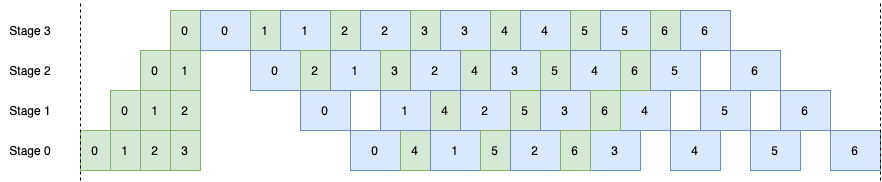
\includegraphics[width=.9\linewidth]{../images/HPGO-Pipeline-no-network.png}
\caption{\label{fig:HPGO-Pipeline-no-network}
Synchronous Pipeline w/out networks}
\end{figure}
\subsubsection{Synchronous Pipelines, w/ networks}
\label{sec:org6220e3c}
\begin{figure}[htbp]
\centering
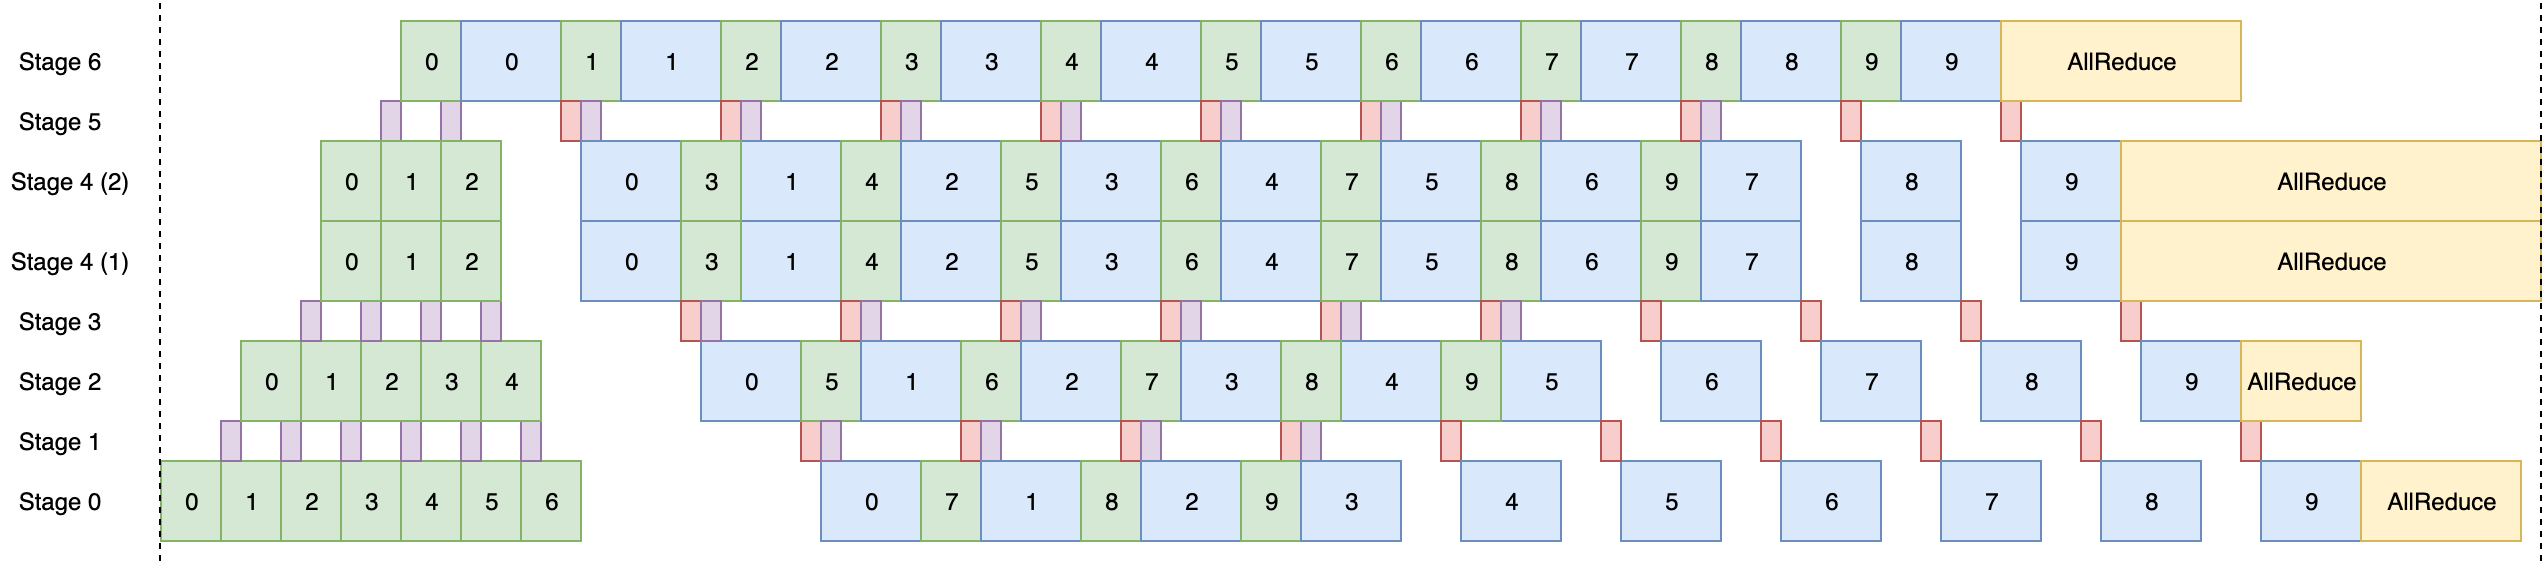
\includegraphics[width=.9\linewidth]{../images/HPGO-Pipeline.png}
\caption{\label{fig:HPGO-Pipeline}
Synchronous Pipeline, where networks are possible bottlenecks}
\end{figure}
\subsubsection{Pipeline Length Calculation}
\label{sec:org8aa1614}
for now we are using a simple approach to estimate the length of a pipeline for every step

\begin{gather}
    PL=\max_{0 \le i < S,\ i\ \%\ 2 == 0} \\\{
    (mBatch \times (FW[Q] + BW[Q]) + \sum_{k=0}^{Q-1}{(FW[k] + BW[k])}) \\- \sum_{s=0}^i BW[s] + \frac{2 \times W_i \times (R_P-1)}{R_P \times B_{slowest}(2 \times W_i \times \frac{R_P-1}{R_P})} \}
\end{gather}

\subsection{Asynchronous Pipelines}
\label{sec:org3cae795}

\section{HPGO v0.8}
\label{sec:orgb81ed4f}
\subsection{Single Pipeline Arrangement}
\label{sec:org507c172}
Assume we already have the optimal device placement, meaning that if a stage is arrange we immediately know which GPU it should run on. 
\subsection{Device Placement}
\label{sec:org30a40d8}

\subsection{Dynamic Programming}
\label{sec:org21a40c0}
\subsection{Proof of Correctness}
\label{sec:org97bc479}
\subsection{Space-Time Complexity}
\label{sec:orgfee4535}

\section{Future Improvements}
\label{sec:orgecc4373}
\end{document}